Double beta decay is a rare nuclear transition in which a nucleus with $Z$ protons decays into a nucleus with $Z+2$ protons and the same mass number $A$. The standard double beta decay mode, the two-neutrino mode \bbtnu, is a second-order weak transition producing two electrons and two antineutrinos, and is allowed in the Standard Model. Despite being a very slow process, it has been observed in a variety of even-even nuclei. The neutrinoless double beta decay mode \bbonu\ is instead a hypothetical process producing two electrons and no neutrinos. While several other processes have been investigated, \bbonu\ is the most promising probe we have in hand to test lepton number violation. Also, a positive result in the search for \bbonu\ would unavoidably indicate that neutrinos are Majorana particles, that is truly neutral particles.  

The experimental exploration of \bbonu\ has a long history, see fig.~\ref{fig:bb0nusearches}. The first search was performed in 1948, where the half-life for \bbonu\ in $^{124}\text{Sn}$ was constrained to be longer than $3\times 10^{15}$ years \cite{Barabash:2011mf}. Half a century later, in 2001, the Heidelberg-Moscow Collaboration reported a half-life limit about ten orders of magnitude more stringent, using \Ge{76} as \bb\ emitter: $T_{1/2}^{0\nu}>1.9\times 10^{25}$ years \cite{Klapdor-Kleingrothaus:2000eir}. It is, also, a history plagued by frequent claimed discoveries (see, for example, \cite{Tretyak:2011pg}) that have been later disproved by subsequent experiments. This observation alone reflects how difficult it is to search for \bbonu.

\begin{figure}[t!b!]
\begin{center}
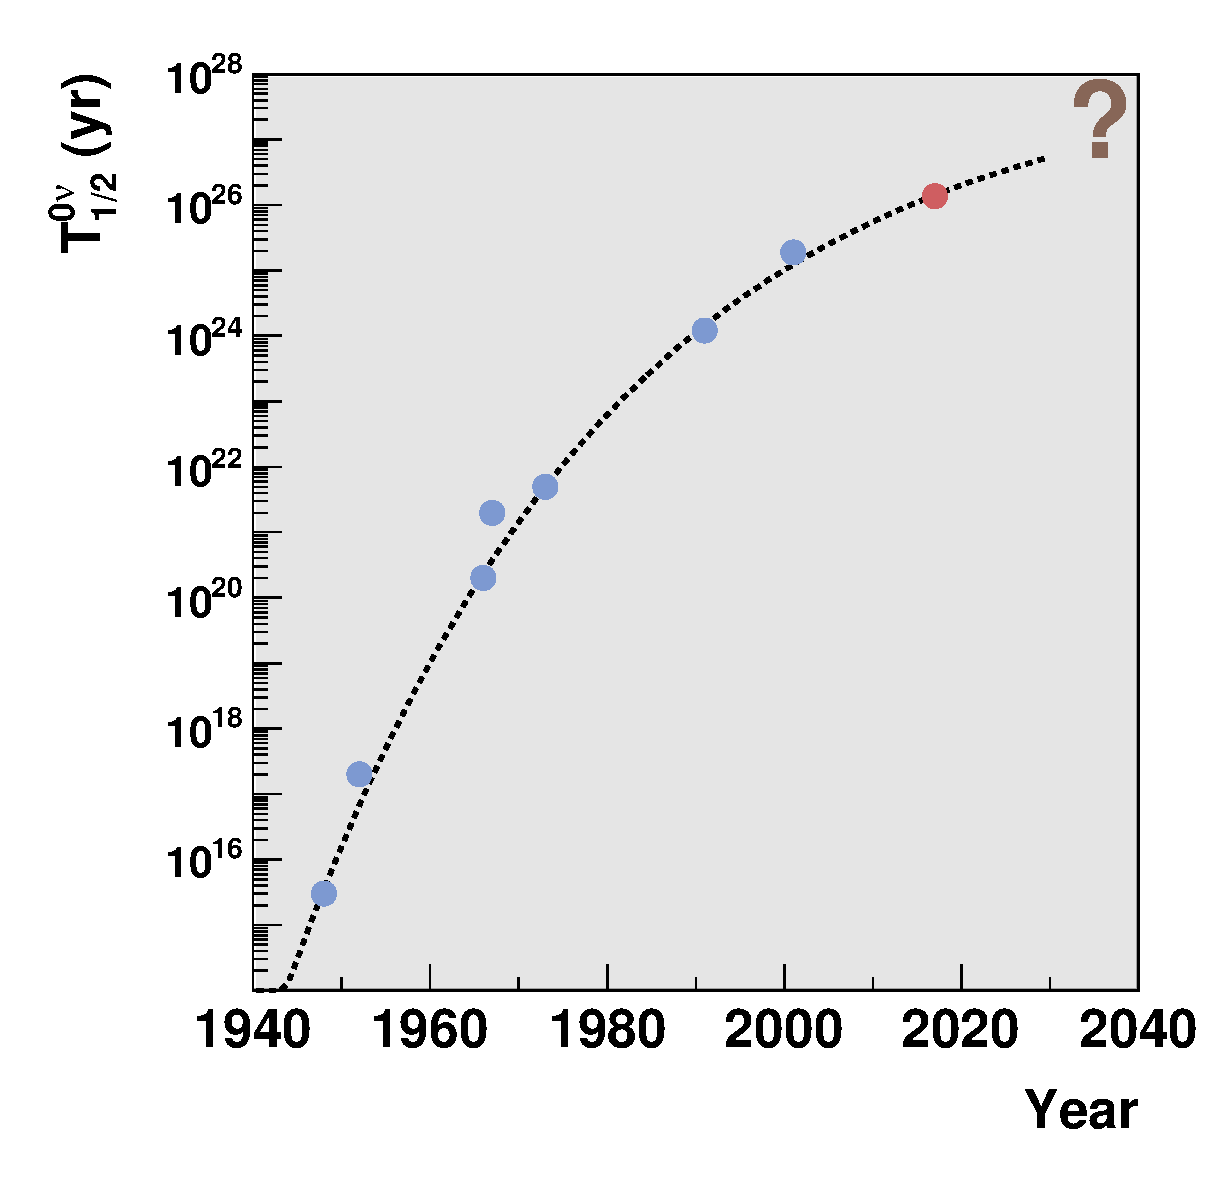
\includegraphics[width=0.70\textwidth]{img/bb0nusearches.eps}
\end{center}
\caption{Seventy years of direct \bbonu\ searches in perspective. Existing limits (shown in blue) are taken from \cite{Barabash:2011mf}. The sensitivity of new-generation proposals (shown in red) is based upon this review, see sect.~\ref{sec:experiments}.} \label{fig:bb0nusearches}
\end{figure}

There is at present a diverse and healthy competition among a variety of experimental techniques to establish themselves as the best approach for \bbonu\ searches. The \bbonu\ field is now witnessing a \emph{golden age} in terms of experimental efforts. Why is that? Some reasons have been present all along during the era of \bbonu\ exploration:
%
\begin{itemize}
%
\item We have a fairly good idea of what to look for. While several mechanisms have been proposed to drive \bbonu, in most of them the two decay electrons are the only light particles emitted, therefore carrying most of the available energy. This can be contrasted with proton decay searches, where it is less clear which decay mode should be the focus of experimental investigation.
%
\item It is common belief that there is still ample room for improvement with respect to the most sensitive \bbonu\ searches performed to date, as can be guessed by the trend in fig.~\ref{fig:bb0nusearches}.
\end{itemize}
%
There are, however, additional reasons that are applicable to the present era: 
\begin{itemize}
\item Probably the most important reason has to do with the discovery of neutrino oscillations over the past two decades, implying that neutrinos are massive particles. If one assumes, as it is customarily done, that light Majorana neutrino exchange is the dominant contribution to \bbonu, there is a direct link between a measurable \bbonu\ rate on the one hand, and the absolute scale of neutrino masses scale and neutrino oscillations phenomenology on the other. In this context, one can also study what is the actual value of neutrino masses, and whether the neutrino mass spectrum exhibits some particular features (such as a hierarchical or a quasi-degenerate structure), via \bbonu. 
%
\item Searching for \bbonu\ is well motivated on theoretical grounds. On the one hand, there is no fundamental reason why total lepton number should be conserved. On the other hand, Majorana neutrinos provide natural explanations for both the smallness of neutrino masses and the baryon asymmetry of the Universe. As a consequence, theoretical prejudice in favor of Majorana neutrinos has gained widespread consensus. 
%
\item As it is well known, there is a $6\ \sigma$ evidence for \bbonu\ in \Ge{76} reported by part of the Heidelberg-Moscow Collaboration, $T_{1/2}^{0\nu}=(2.23^{+0.44}_{-0.31})\times 10^{25}$ years \cite{Klapdor-Kleingrothaus:2006zcr}. It is also well known that this claim is highly controversial \cite{Aalseth:2002dt}. Consensus exists that the issue can only be definitely settled by new, and more sensitive, experiments.
\end{itemize}

The mapping of observed \bbonu\ rates into neutrino mass constraints not only requires assuming the standard \bbonu\ interpretation in terms of light Majorana neutrino exchange. It also requires precise nuclear physics knowledge, which can be factorized into the so-called nuclear matrix elements (NMEs). These NMEs cannot be measured, and need to be separately calculated for each \bb\ emitting isotope under consideration. Several calculations exist. While they share common ingredients, calculations differ in their treatment of nuclear structure. We argue that about a 20-30\% NME uncertainty exists for converting rates into neutrino masses. 

In this review, the different experimental aspects affecting \bbonu\ searches were extensively discussed. The requirements are often conflicting, and no new-generation experimental proposal is capable of optimizing all of them. Should we concentrate on approaches offering huge event rates, such as KamLAND-Zen? Are superior energy resolution techniques, such as GERDA or CUORE, the best way to go? Should background suppression focus more on radiopurity control, as in the EXO or KamLAND-Zen cases, or on powerful signal-background discrimination techniques, as in the SuperNEMO or NEXT approaches? We made an attempt at a quantitative comparison of the physics case of selected new-generation experimental approaches, which is summarized in fig.~\ref{fig:sens-pmr}. 

What about the longer-term future? How far can we go in \bbonu\ exploration? Nobody knows for sure. What we do know is that such future \bbonu\ searches will unavoidably need to involve experiments at the ton or multi-ton scale in \bb\ isotope mass. The diversity of experimental approaches we are currently witnessing will not be viable at that scale, and 2 or 3 approaches (most likely based on different isotopes) are going to be retained at most. However, an extrapolation of the trends from the past and the present may offer some qualitative clues. Figure~\ref{fig:bb0nusearches} seems to point to ``asymptotic'' limits of \bbonu\ half-life explorations in the $10^{28}$ years range. If the light Majorana neutrino exchange mechanism is realized in Nature, this would correspond to effective Majorana masses at the few meV scale. As can be appreciated in fig.~\ref{fig:mbetabetavsmlight}, such ultimate \bbonu\ sensitivities would give us good chances to detect \bbonu\ regardless of the value of the neutrino mass and mixing parameters. 

An unambiguous detection, either in the current-generation efforts starting now or in the longer-term future, would open up an even more exciting era for \bbonu\ searches, with the objective to actually understand what is the physics mechanism that is responsible for this elusive process.



  

